\documentclass[../thesis.tex]{subfiles}

\begin{document}
\section{Application Architecture}

\subsection{Architectural Design}
\begin{figure}[H]
    \centering
    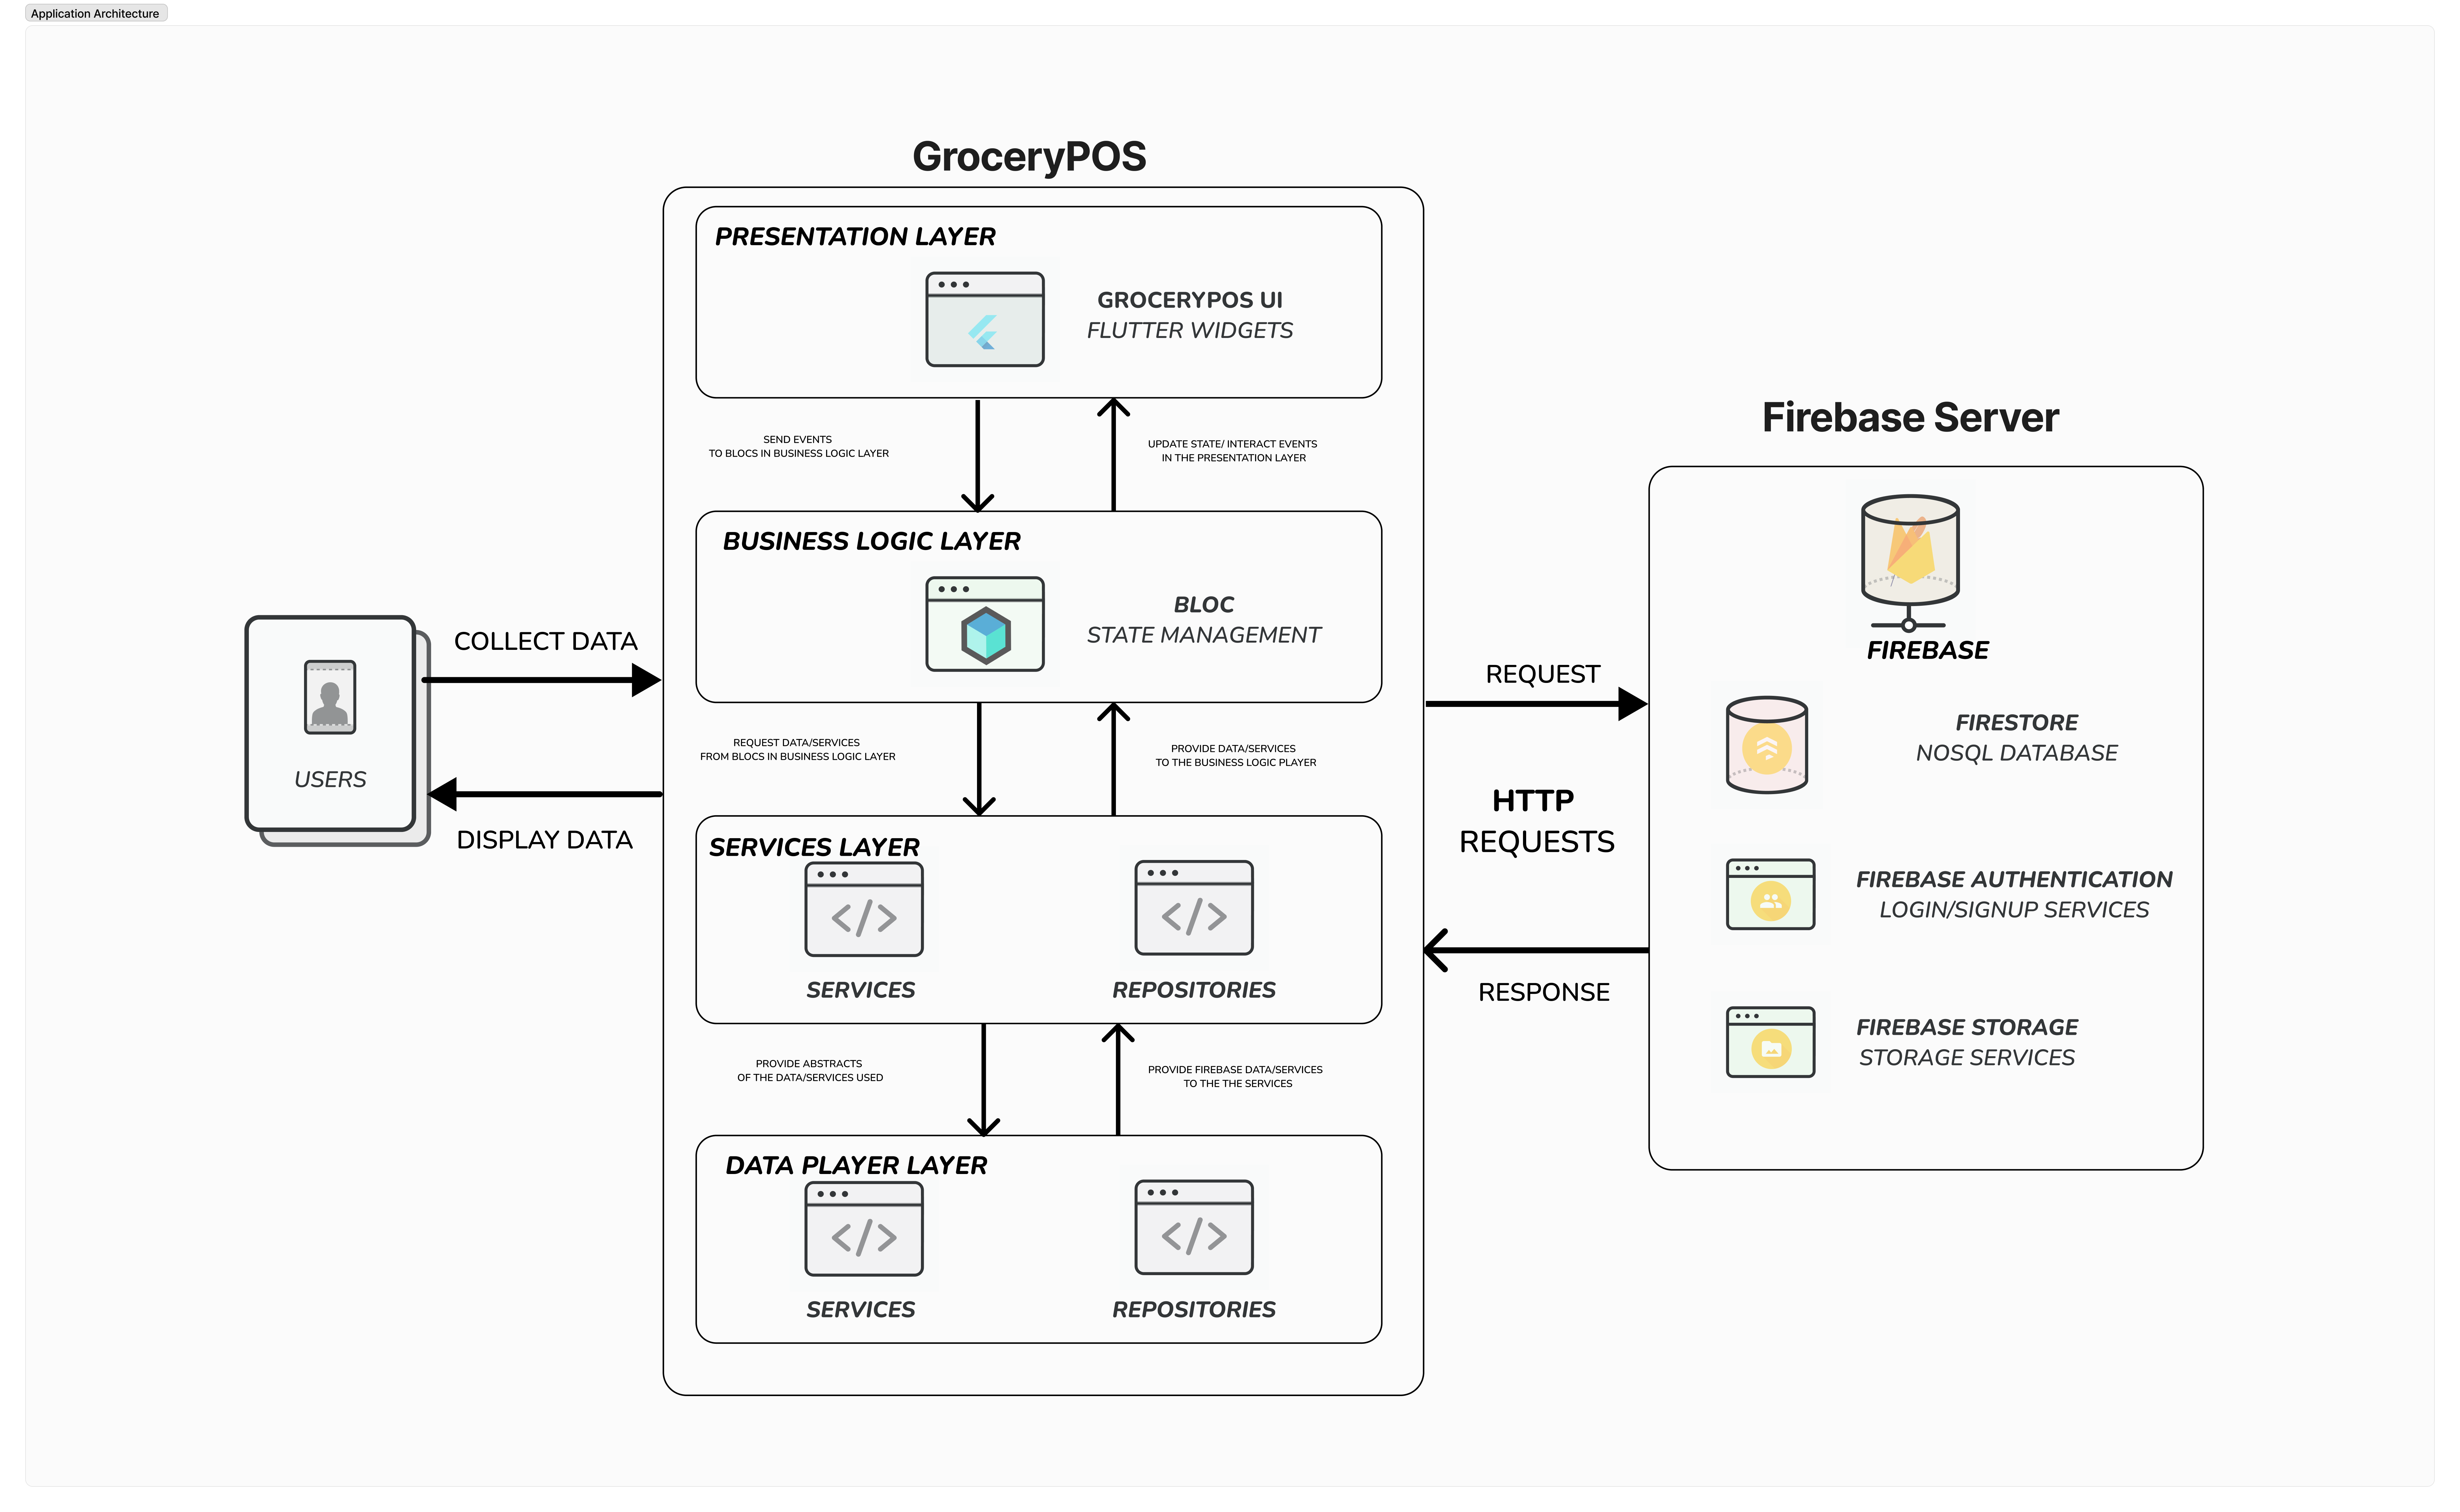
\includegraphics[width=1\textwidth]{images/Application-Architecture.png}
    \caption{Application Architecture}
    \label{fig:application-architecture}
\end{figure}
\subsection{Decomposition Description}
\begin{figure}[H]
    \centering
    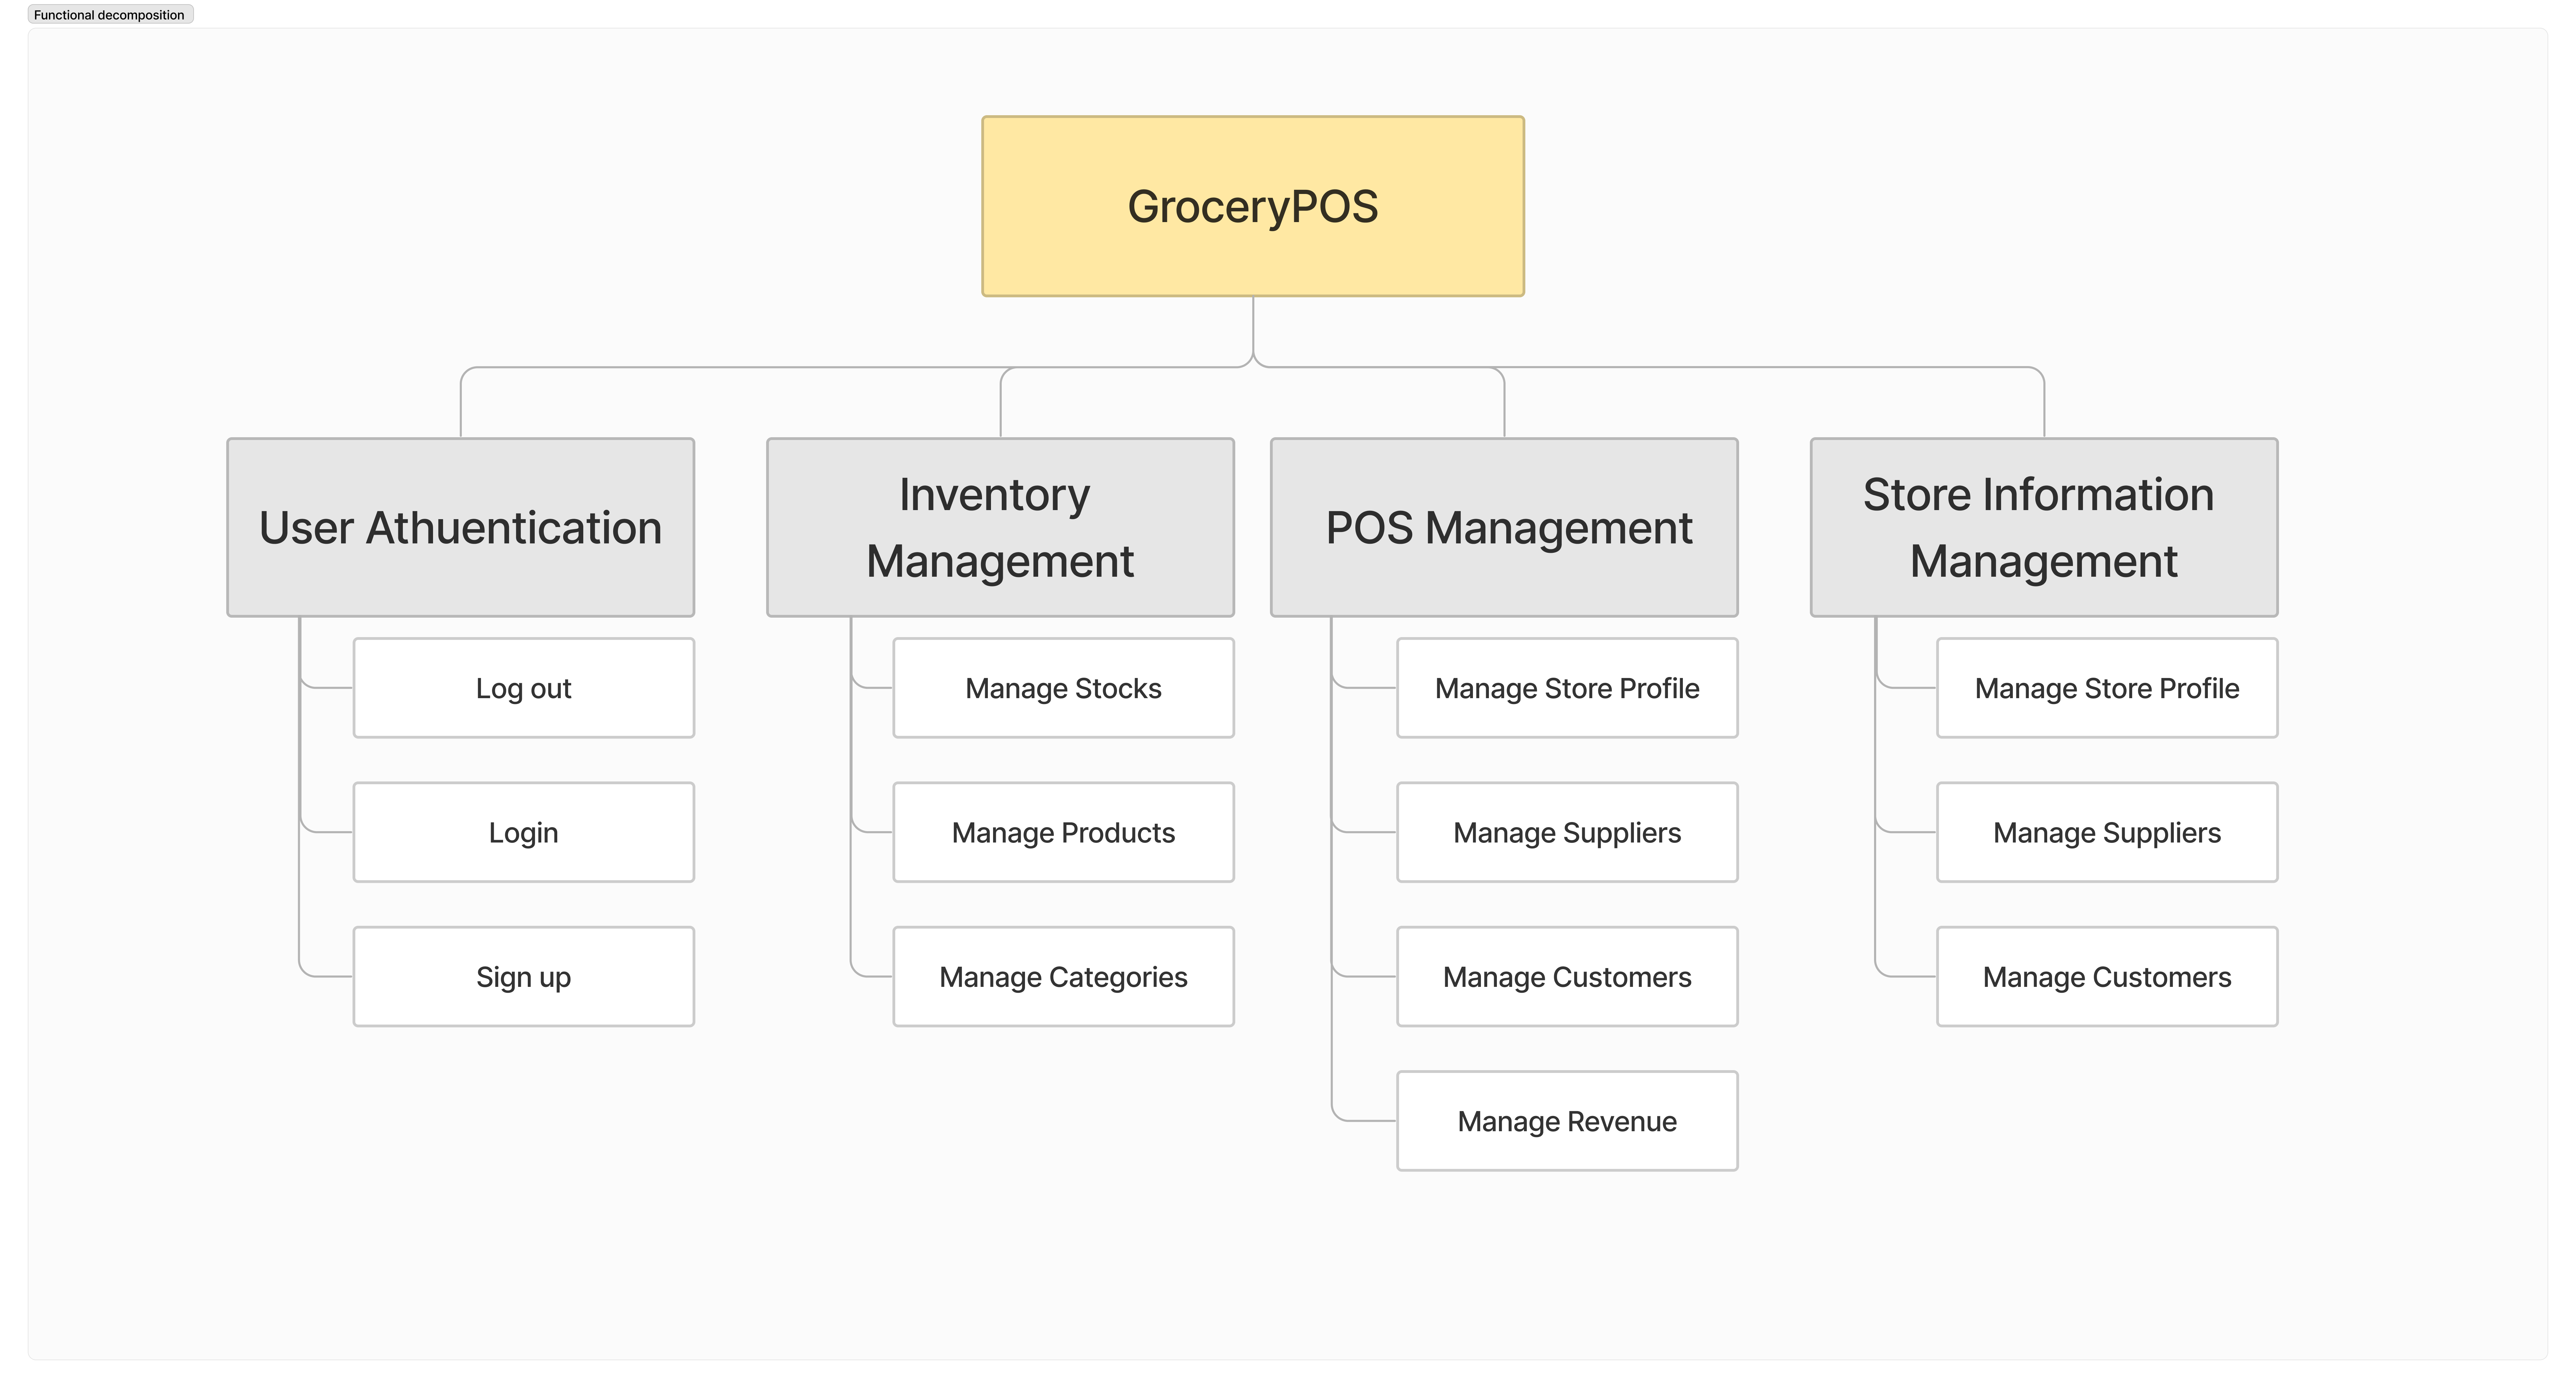
\includegraphics[width=1\textwidth]{images/Functional-Decomposition.png}
    \caption{Decomposition Description}
    \label{fig:functional-decomposition}
\end{figure}
% System
% |
% |-- User Authentication
% |   |-- Login
% |   |-- Logout
% |
% |-- Inventory Management
% |   |-- Inventory Tracking
% |   |-- Product Management
% |   |   |-- Add Product
% |   |   |-- Edit Product
% |   |   |-- Delete Product
% |   |
% |   |-- Category Management
% |
% |-- Sales Management
% |   |-- Invoice Creation
% |   |-- Invoice Management
% |   |   |-- View Invoice
% |   |   |-- Edit Invoice
% |   |   |-- Delete Invoice
% |   |
% |   |-- Invoice Printing
% |   |-- Revenue and Expenditure Management
% |
% |-- Store Information Management
%     |-- Supplier Management
%     |   |-- Add Supplier
%     |   |-- Edit Supplier
%     |   |-- Delete Supplier
%     |
%     |-- Customer Management
%         |-- Add Customer
%         |-- Edit Customer
%         |-- Delete Customer

% \subsection{Design Basis}
\section{Data Design}
\subsection{Data Description}
\subsubsection{Conceptual Data Model}
\subsubsection{Logical Data Model}
\subsubsection{Physical Data Model}
\subsection{Data Dictionary}
\section{Detailed Design}
\end{document}